\documentclass[a4paper,12pt]{article}
\usepackage{geometry}
\geometry{left=2.5cm, right=1.0cm, top=2.0cm, bottom=2.0cm}
\usepackage[T2A]{fontenc}
\usepackage[utf8]{inputenc}
\usepackage[russian,english]{babel}
\usepackage{amsmath}
\usepackage{amssymb}
\usepackage{graphicx}
\usepackage{float}
\usepackage{setspace}
\usepackage{indentfirst}
\usepackage{comment}
\usepackage[
backend=biber,
style=numeric,
urldate=long,
maxbibnames=99
]{biblatex}
\addbibresource{refs.bib}
\usepackage[colorlinks=true, citecolor=blue, linkcolor=blue, urlcolor=blue, pdfstartview=FitH]{hyperref}
\usepackage{mathtools}
\usepackage{booktabs}

\usepackage{chngcntr}
\counterwithin{table}{section}
\counterwithin{figure}{section}

\graphicspath{{graphics/}}

\setlength{\parindent}{1.25cm}
\renewcommand{\baselinestretch}{1.5}

\newcommand{\bibref}[3]{\hyperlink{#1}{#2 (#3)}}

\renewcommand{\theenumi}{\arabic{enumi}}
\renewcommand{\labelenumi}{\arabic{enumi}.}
\renewcommand{\theenumii}{.\arabic{enumii}}
\renewcommand{\labelenumii}{\arabic{enumi}.\arabic{enumii}.}
\renewcommand{\theenumiii}{.\arabic{enumiii}}
\renewcommand{\labelenumiii}{\arabic{enumi}.\arabic{enumii}.\arabic{enumiii}.}

\begin{document}
\begin{titlepage}
\newpage
{\setstretch{1.0}
\begin{center}
NATIONAL RESEARCH UNIVERSITY\\
HIGHER SCHOOL OF ECONOMICS
\\
\bigskip
Faculty of Computer Science\\
Bachelor's Programme "Data Science and Business Analytics"
\end{center}
}
\vspace{4em}
\begin{center}
{\bf Software Project Report on the Topic:}\\
{\bf A VQA-Augmented Multimodal Meme Retrieval System}\\
(interim, the first stage)
\end{center}

\vspace{6em}
{\bf Submitted by the Student: \vspace{2mm}}

{\setstretch{1.1}
\begin{tabular}{l@{\hskip 1.5cm}l}
group \#\foreignlanguage{russian}{БПАД}233, 3rd year of study \\
Khamidullin Amir Aydarovich \\
\end{tabular}}

\vspace{1em}
{\bf Approved by the Project Supervisor: \vspace{2mm}}

{\setstretch{1.1}
\begin{tabular}{l@{\hskip 1.5cm}l}
Burlova Albina Sergeevna\\
Senior lecturer\\
Faculty of Computer Science, HSE University 
\end{tabular}}

\vspace{\fill}
\begin{center}
Moscow 2026
\end{center}
\end{titlepage}

\newpage
\setcounter{page}{2}

{
	\hypersetup{linkcolor=black}
	\tableofcontents
}

\newpage

%==============================================================================
% ANNOTATION
%==============================================================================
\section*{Annotation} 
\addcontentsline{toc}{section}{Annotation}
This work presents an intelligent multimodal meme retrieval system implemented
as a Telegram bot, enabling users to find relevant memes by text description
(in English or Russian), by reference image, or by their combination.
The system uses GPT with vision capabilities to generate structured 10-field
annotations for each meme, the BGE-M3 multilingual encoder to build three FAISS
indices, and Reciprocal Rank Fusion (RRF) for late fusion of search results.
Maximal Marginal Relevance (MMR) ensures diversity in the output.
The corpus contains 16,030 annotated memes from 6 sources, with 5,827 exact
duplicates identified via perceptual hashing and filtered at retrieval time.
On a test set of 100 memes (495 queries), the system achieves
Hit@5 = 60.0\% for English and 57.0\% for Russian queries.


\section*{\foreignlanguage{russian}{Аннотация}}
\foreignlanguage{russian}{
В данной работе представлена интеллектуальная система мультимодального поиска мемов, реализованная в виде Telegram-бота. Система позволяет находить релевантные мемы по текстовому описанию на английском или русском языке, по референсной картинке, либо по их комбинации. Для аннотации используется визуально-языковая модель GPT, генерирующая 10 структурированных полей для каждого мема. Мультиязычный энкодер BGE-M3 строит три FAISS-индекса, результаты объединяются через Reciprocal Rank Fusion (RRF). Для обеспечения разнообразия выдачи применяется Maximal Marginal Relevance (MMR). Корпус содержит 16~030 аннотированных мемов из 6 источников, из которых 5~827 точных дубликатов выявлены перцептивным хешированием и исключены из выдачи. На тестовой выборке из 100 мемов (495 запросов) система достигает Hit@5 = 60.0\% для английских и 57.0\% для русских запросов.
}

\section*{Keywords}
Multimodal retrieval, VQA, vision-language models, BGE-M3, FAISS, RRF, MMR, perceptual hashing, memes, Telegram bot

\pagebreak

%==============================================================================
% INTRODUCTION
%==============================================================================
\section{Introduction}
\subsection{Motivation and Relevance}

In the modern digital landscape, internet memes have become a universal means of communication, combining visual content and text to convey cultural context, humor, and social commentary. According to various studies, millions of new memes are created daily, and their use spans all areas of online communication—from personal messaging to marketing campaigns.

However, existing image search tools are insufficiently effective for working with memes. Standard search engines are oriented toward keyword-based or visual similarity search, which does not account for the specifics of memes as multimodal content. The main challenges include the following:

\begin{enumerate}
    \item Semantic complexity: a meme often contains hidden meaning that cannot be derived directly from the visual content or text separately. Understanding a meme requires joint analysis of the image and overlaid text.
    
    \item Cultural context: meme interpretation presupposes knowledge of cultural references, internet trends, and the specifics of online communities. The same template can be used to convey completely different messages.
    
    \item Format diversity: memes range from simple images with text to complex collages and comics, which complicates the application of unified processing methods.
\end{enumerate}

The emergence of multimodal machine learning models, such as CLIP~\cite{radford2021clip}, opens new opportunities for solving the meme retrieval task. These models can create a unified vector representation for text and images, enabling cross-modal search.
\subsection{Project Goal and Objectives}

The goal of this project is to develop an intelligent multimodal meme retrieval service, implemented as a Telegram bot with a backend system, that allows users to find relevant memes by text description, reference image, or their combination.

To achieve this goal, the following objectives must be accomplished:

1. Collect and prepare a database of approximately 16,000 memes from open sources, including text extraction from images (OCR) and semantic description generation using a vision-language model (GPT with 10 structured annotation fields).

2. Build a multimodal index based on vector embeddings (BGE-M3) with efficient storage and search organization in FAISS.

3. Implement a hybrid retrieval architecture with Reciprocal Rank Fusion (RRF) of multiple indices and Maximal Marginal Relevance (MMR) for result diversity.

4. Develop a Telegram bot supporting three input modes (text, image, hybrid) with a user-friendly interface and automatic database updates.

5. Conduct system quality evaluation using information retrieval metrics on a validation set with manual annotation.

\subsection{Practical Significance}

The developed system has practical value for a wide range of users. Regular users will get a convenient tool for quickly finding the right memes in everyday communication. SMM specialists and content managers will be able to promptly find relevant visual content for publications. Researchers of internet culture will receive a tool for analyzing and systematizing memes.

Additionally, the architectural solutions and methods developed within this project can be applied to other multimodal image retrieval tasks.

\subsection{Novelty}

The novelty of this project lies in its comprehensive approach to multimodal meme retrieval, which includes:

1. Use of VQA annotations: applying GPT with vision to generate structured 10-field meme descriptions that account for visual content, overlaid text, semantics, emotions, and search queries. Unlike simple captioning, this approach captures deeper semantic information.

2. Hybrid retrieval architecture: combining early fusion (all annotation fields concatenated before encoding) with late fusion (RRF across multiple FAISS indices after independent search). Maximal Marginal Relevance (MMR) ensures diversity in the final ranking.

3. Corpus deduplication: applying perceptual hashing (phash) to detect cross-source duplicates, which are filtered at retrieval time while preserving index position consistency.

4. Specialization for the meme domain: adapting approaches to the specifics of internet memes, which differ from standard images by having overlaid text, cultural references, and semantic complexity.

\pagebreak

%==============================================================================
% LITERATURE REVIEW
%==============================================================================

\section{Literature Review}

From existing works in multimodal image retrieval, several key directions can be identified: building a shared embedding space for text and images, generating descriptions using vision-language models, meme understanding as a separate task, and efficient vector search methods.

A breakthrough in multimodal learning came with the CLIP model, presented in the work by \href{https://arxiv.org/abs/2103.00020}{Radford et al. (2021)}. The authors trained a pair of neural network encoders: Vision Transformer for images and Transformer for text on 400 million text-image pairs collected from the internet. The model creates a unified vector space where semantically similar texts and images are located close together. This enables cross-modal search using cosine similarity. However, CLIP was trained on general images and does not account for meme specifics—overlaid text, cultural references, and multi-layered humor.

For generating textual descriptions of images, vision-language models have been developed. The work by \href{https://arxiv.org/abs/2301.12597}{Li et al. (2023)} presents the BLIP-2 model, which uses the Q-Former architecture to efficiently bridge frozen visual encoders with large language models. The model achieves state-of-the-art results on VQA and image captioning tasks with significantly lower computational costs. An alternative approach is proposed in the work by \href{https://arxiv.org/abs/2304.08485}{Liu et al. (2023)}, where the LLaVA model is trained to follow natural language instructions when working with images. This allows flexible query formulation for extracting specific information from images. In this project, VLMs will be used to generate VQA annotations—structured meme descriptions.

The task of automatic meme understanding is studied in several works. In the work by \href{https://arxiv.org/abs/2005.04790}{Kiela et al. (2020)}, as part of the Hateful Memes Challenge, a dataset of 10,000 memes was created, specifically designed so that neither text nor image alone would allow determining whether a meme is offensive. Results showed that multimodal models (64.7\% accuracy) significantly outperform unimodal ones (59.2\% for text, 52.6\% for images), confirming the necessity of joint analysis. The work by \href{https://aclanthology.org/2024.findings-acl.246/}{Roy et al. (2024)} extends this direction by presenting the MemeMQA dataset for question-answering interaction with memes. However, both works focus on classification rather than meme retrieval.

Efficient embedding-based search requires specialized data structures. The FAISS library, described in the work by \href{https://arxiv.org/abs/2401.08281}{Douze et al. (2024)}, provides optimized implementations of IVF and Product Quantization algorithms, ensuring sub-millisecond search latency on billion-scale collections. The HNSW algorithm, presented in the work by \href{https://arxiv.org/abs/1603.09320}{Malkov \& Yashunin (2020)}, uses a hierarchical graph structure to achieve logarithmic search complexity.

Modern information retrieval systems combine different ranking methods. The work by \href{https://aclanthology.org/2021.tacl-1.20/}{Luan et al. (2021)} provides a systematic analysis of sparse (BM25) and dense (neural) representations, showing that a hybrid approach outperforms each method individually by 5-8\% on the MRR@10 metric. To improve result precision, re-ranking is applied. The work by \href{https://arxiv.org/abs/2004.12832}{Khattab \& Zaharia (2020)} presents the ColBERT model with a late interaction mechanism, providing cross-encoder quality at 170x higher speed.

For extracting text from memes, OCR systems are required. The work by \href{https://arxiv.org/abs/2009.09941}{Du et al. (2020)} presents the PaddleOCR system, achieving 90.3\% accuracy on text detection and providing 10x faster speed than Tesseract on images with complex backgrounds.

Thus, existing image search solutions do not account for the multimodal nature of memes, while academic works on meme understanding focus on classification rather than retrieval. This project combines multimodal embeddings, VQA annotations, hybrid search, and re-ranking into a unified system specifically for the meme retrieval task.

\pagebreak

%==============================================================================
% WORK PLAN
%==============================================================================
\section{Work Plan}

\begin{table}[h!]
\centering
\begin{tabular}{|l|l|p{8cm}|}
\hline
\textbf{Period} & \textbf{Phase} & \textbf{Key Deliverables} \\
\hline
Jan 2026 & Data Collection & Database of 18,000+ memes from 6 sources \\
\hline
Feb 2026 & Data Processing & Two-stage OCR + VQA annotations via Qwen2.5-VL \\
\hline
Mar 2026 & Index Building & CLIP + text embeddings, FAISS index, BM25 index \\
\hline
Apr 2026 & System Development & FastAPI backend + Telegram bot with 3 search modes \\
\hline
May 2026 & Finalization & Load/latency stress tests, monitoring + final report \\
\hline
\end{tabular}
\caption{Project timeline}
\end{table}

\vspace{0.5cm}

\textbf{Phase 1: Data Collection \& Cleaning.} Parsing memes from Bing Images, Telegram sticker packs, Kaggle datasets, HuggingFace, and Imgflip. Filtering duplicates and inappropriate content using content moderation lists.

Phase 2: Annotation Pipeline. Two-stage OCR (EasyOCR + PaddleOCR v3) with confidence-based filtering. Initial VQA annotations using Qwen2.5-VL-3B via Ollama (4 fields), followed by re-annotation with GPT Vision (10 fields) for the full corpus.

Phase 3: Search Infrastructure. Computing bge-m3 embeddings for text. Building 3 FAISS indices (mega-text, EN search queries, RU search queries). Perceptual hash deduplication.

Phase 4: Application Layer. Telegram bot (aiogram 3) supporting text, image, and hybrid queries. GPT Vision for image-based search. RRF fusion and MMR diversity.

\textbf{Phase 5: Finalization.} Quality evaluation (Hit@K, MRR@10) on 100 annotated memes (495 queries), final report preparation.
\pagebreak

%==============================================================================
% METHODOLOGY
%==============================================================================
\section{Methodology}

This chapter describes the methodology of the project: the process of building the meme corpus, the VQA annotation pipeline, and the system architecture for multimodal retrieval.

\subsection{Data Collection}

To build a diverse meme corpus covering different formats, languages, and cultural contexts, images were collected from six sources, as summarized in Table~\ref{tab:sources}.

\begin{table}[h!]
\centering
\begin{tabular}{|l|l|r|}
\hline
\textbf{Source} & \textbf{Method} & \textbf{Images} \\
\hline
Bing Images & Custom scraper with query rotation & 6,142 \\
\hline
Telegram Stickers & Automated sticker pack extraction & 4,382 \\
\hline
Kaggle Memotion & Manual download (competition dataset) & 6,969 \\
\hline
Kaggle Russian Memes & Manual download & 675 \\
\hline
HuggingFace Datasets & API download script & 330 \\
\hline
Imgflip (575k subset) & Template-based download & 390 \\
\hline
\textbf{Total (raw)} & & \textbf{18,888} \\
\hline
\end{tabular}
\caption{Data sources and collection statistics}
\label{tab:sources}
\end{table}

The Bing Images scraper uses query rotation with 50+ search terms covering popular meme categories (e.g., ``funny memes'', ``reaction images'', ``dank memes'') and downloads images in parallel with deduplication by URL hash. The Telegram sticker extractor processes public sticker packs, converting WebP stickers to JPEG format. All images are saved in their original resolution with supported formats: JPEG, PNG, and WebP.

\subsubsection{OCR Pipeline}

Text extraction from meme images is performed using two OCR engines in a cascaded configuration.

Stage 1: EasyOCR. The initial pass uses the EasyOCR library with Russian and English language models. For each image, the system extracts detected text segments along with their confidence scores. Results are stored as \texttt{metadata\_ocr.csv}.

Stage 2: PaddleOCR v3. Images that passed the first cleaning stage are processed by PaddleOCR v3~\cite{du2020ppocr} with Russian language support. PaddleOCR employs the DB text detector and CRNN-based recognizer, providing complementary recognition results. Images are read via OpenCV to handle all formats including WebP.

Design choice: cascade vs ensemble. A parallel ensemble approach---running both engines on every image and selecting the best result---would reduce error propagation but would double processing time and require a pre-labelled alignment set to weight engine outputs reliably. Given the hardware constraints (Apple M4 Pro, 24~GB unified RAM) and the project timeline, the cascaded design was preferred: EasyOCR provides a fast initial quality gate, and PaddleOCR refines the surviving subset. This trades some recall for significantly lower total runtime (approximately 3~hours vs 6~hours for 16,000 images). An ensemble re-run is planned as a future improvement.

Confidence threshold. The 0.6 threshold was selected after manual inspection of approximately 150 PaddleOCR outputs. At confidence $\geq 0.6$, outputs were found to be usable as-is in more than 90\% of spot-checked cases.

\subsubsection{Data Cleaning and Filtering}

The cleaning pipeline operates in two passes with different filter configurations.

Pass 1: EasyOCR cleaning. The first pass filters entries by content and text quality:
\begin{enumerate}
    \item Content moderation: A curated list of 580+ prohibited words and phrases in Russian and English. Matching is performed via exact substring search with an additional fuzzy matching step using the Levenshtein distance, with a similarity threshold of 85\%.
    \item Text length constraints: Minimum text length of 3 characters, maximum of 400 characters.
\end{enumerate}

Pass 2: PaddleOCR merge and final filtering. PaddleOCR results from all data sources are merged into a single dataset with a confidence-based filter:
\begin{enumerate}
    \item Confidence filtering: Entries with OCR text longer than 2 characters but confidence below 0.6 are removed. Entries with zero confidence or confidence $\geq 0.6$ are retained. The threshold of 0.6 was chosen empirically after manual inspection of PaddleOCR outputs: below this value, the recognized text frequently contains character substitutions, merged words, and spurious characters that would introduce noise into downstream VQA annotations.
    \item Content moderation: A second pass of bad-word filtering using exact substring matching.
\end{enumerate}

It should be noted that the confidence score in OCR systems is an empirical measure of recognition quality for a detected character sequence, not a reliable indicator of text presence. A confidence of 0 may indicate a recognition failure rather than the absence of text. Proper threshold calibration requires a labelled dataset of 200--500 manually annotated memes with transcriptions, measured by CER, WER, and precision/recall. This validation is planned for the next stage.

\subsubsection{Final Dataset}

After merging results from both OCR engines and applying all filters, the final dataset contains 16,080 entries from 18,888 raw images. A total of 539 images were removed by the content moderation filter, and the remaining were filtered by confidence and text quality.

Each entry in the final dataset contains: \texttt{filename}, \texttt{source\_path}, \texttt{ocr\_text}, \texttt{confidence}, and \texttt{source\_type}.

\pagebreak

%==============================================================================
% VQA ANNOTATION PIPELINE
%==============================================================================
\subsection{VQA Annotation Pipeline}

To enable semantic meme retrieval beyond simple text or visual similarity, each meme requires a structured semantic description. This section describes the VQA annotation pipeline that generates these descriptions automatically using a vision-language model.

\subsubsection{Model Selection}

Several vision-language models were considered for the VQA annotation task. The initial prototype used Qwen2.5-VL-3B running locally via Ollama on Apple M4 Pro (24~GB unified RAM). While this model produced acceptable results for an initial subset of 10,000 memes, it was limited by processing speed (2--4 seconds per image), an approximately 3.3\% hallucination rate, and coverage of only 4 fields per pass (caption, objects, tone, main\_idea), requiring a separate enrichment stage.

For the final annotation run, the pipeline was migrated to GPT with vision capabilities (via an OpenAI-compatible API endpoint). This enabled:

\begin{itemize}
    \item A single-pass annotation producing all 10 structured fields simultaneously.
    \item Significantly higher output quality with near-zero hallucination rate.
    \item Parallel processing with 5 concurrent workers, completing 16,030 memes in approximately 4 hours.
\end{itemize}

\subsubsection{Subset Selection for Annotation}

From the 16,080 cleaned entries, all images were selected for VQA annotation (no subset sampling was required due to the efficiency of the GPT-based pipeline). The final annotated corpus contains 16,030 memes (50 images were skipped due to file corruption or format issues).

\subsubsection{Annotation Schema}

The annotation pipeline operates in a single pass, producing a rich structured representation for each meme.

The \texttt{annotate\_memes.py} script processes each meme image through GPT with vision and produces a complete annotation in JSON format with 10 fields:

\begin{itemize}
    \item \texttt{caption}: A 1--2 sentence neutral description of the image content.
    \item \texttt{ocr\_text}: Text extracted from the image by the VLM.
    \item \texttt{meme\_template}: Name of the recognized meme template (e.g., Drake, Distracted Boyfriend).
    \item \texttt{objects}: A list of up to 5 key visual objects.
    \item \texttt{tone}: The emotional tone (ironic, wholesome, absurd, dark, relatable, aggressive, neutral).
    \item \texttt{main\_idea}: One sentence summarizing the joke or main message.
    \item \texttt{search\_queries}: 3--5 natural-language search queries that would lead to this meme.
    \item \texttt{tags}: 5--10 descriptive tags.
    \item \texttt{emotions}: List of emotions conveyed.
    \item \texttt{vqa}: 3 question--answer pairs covering text content, scene description, and joke explanation.
\end{itemize}

Images are resized to 512px maximum dimension and converted to JPEG before encoding to base64. The model is queried with \texttt{temperature=0.2} and an 800-token generation limit.

\subsubsection{Pipeline Implementation}

The script supports resume functionality via \texttt{load\_already\_processed()}: it tracks already-processed filenames and skips them on restart. Processing is parallelized with \texttt{ThreadPoolExecutor(5 workers)}. JSON response parsing includes robust handling of markdown code blocks and truncated responses.

All annotations are stored in JSONL format (\texttt{vqa\_annotations\_v3.jsonl}), with one JSON object per line. Each record contains the 10 VQA fields plus metadata: \texttt{filename}, \texttt{source\_path}, \texttt{confidence}, \texttt{source\_type}, \texttt{is\_nsfw}, \texttt{is\_duplicate}, and \texttt{search\_queries\_ru} (Russian translations of search queries).

\pagebreak

%==============================================================================
% SYSTEM ARCHITECTURE
%==============================================================================
\subsection{System Architecture}
\label{sec:arch}

This section describes the overall architecture of the multimodal meme retrieval system, including the embedding generation pipeline, index construction, and the planned search interface.

\subsubsection{Embedding Generation}

The system generates dense vector embeddings per meme using a single multilingual sentence transformer.

Text embeddings (BGE-M3). All 10 textual annotation fields are combined into a unified representation using the \texttt{BAAI/bge-m3} multilingual sentence transformer~\cite{chen2024bge}, producing 1024-dimensional normalized vectors. This model supports 100+ languages including English, Russian, and Chinese.

The choice of bge-m3 over \texttt{all-MiniLM-L6-v2} (the initial baseline) was made after a systematic comparison of 8 multilingual models (Section~\ref{sec:model_exp}). bge-m3 demonstrated the best EN/RU balance: Hit@5 increased from 32\% to 39\% for English queries and from 2\% to 37\% for Russian queries.

\subsubsection{Index Construction}

For fast nearest neighbor search, the system builds FAISS~\cite{douze2024faiss} indices using \texttt{IndexFlatIP} (inner product on L2-normalised vectors, equivalent to cosine similarity). Three indices are constructed:

\begin{itemize}
    \item \texttt{faiss\_C\_all.index}: 1024-dimensional, all 10 annotation fields concatenated into a single mega-text (early fusion), encoded with bge-m3.
    \item \texttt{faiss\_D\_search\_queries.index}: 1024-dimensional, English search queries only (bge-m3).
    \item \texttt{faiss\_ru\_search\_queries.index}: 1024-dimensional, Russian-translated search queries (bge-m3).
\end{itemize}

All indices contain 16,030 vectors. A metadata JSONL file maps index positions to filenames, source paths, and all annotation fields.

\subsubsection{Search Modes}

The system supports three retrieval modes:

\begin{enumerate}
    \item Text search (EN/RU): The query is encoded with bge-m3 and searched across multiple indices. For English queries, two indices are used (C mega-text + EN search queries) with RRF fusion (weights 0.6, 0.4). For Russian queries (detected by Cyrillic character presence), all three indices are used (C + EN + RU) with weights 0.4, 0.3, 0.3. After RRF fusion, Maximal Marginal Relevance (MMR) removes results with cosine similarity $>0.80$ to already-selected items, ensuring diverse output.
    
    \item Image search: The user uploads a reference image, which is analysed by GPT with vision capabilities to generate a textual description. This description is then used as a text query through the standard retrieval pipeline, enabling semantic image-based search without a dedicated image embedding index.
    
    \item Hybrid search: The user sends an image with a text caption. Both signals are processed independently—text query through the standard pipeline and image through GPT Vision captioning—and results are fused using a second-level RRF with weights 0.6 (text) and 0.4 (image).
\end{enumerate}

\subsubsection{Application Layer}

The user-facing application is a Telegram bot built with the aiogram~3 framework. The bot loads 3 FAISS indices, the BGE-M3 model, and all meme metadata at startup. It supports text queries in English and Russian, image-based search (via GPT Vision), hybrid search (image + text), paginated results (5 memes per page, up to 25 total), and automatic database updates. A background task checks the \texttt{data/raw/new/} directory every 5 minutes for new memes, processes them through the full annotation pipeline (GPT + translation + encoding), and adds them to the live indices without restarting the bot. When the database exceeds a configurable limit, a cluster-based rotation removes the oldest memes proportionally across tag categories to prevent distribution drift.

For image-based search, uploaded photos are analysed by GPT Vision to generate a caption, then perceptual hashing (phash, 256-bit) is used to exclude the query image itself and near-duplicates from the results.

\pagebreak

%==============================================================================
% CURRENT RESULTS
%==============================================================================
\section{Current Results}

This chapter summarizes the results achieved during the project (as of May 2026).

\subsection{Dataset Summary}

Table~\ref{tab:dataset} presents the final dataset statistics after all preprocessing stages.

\begin{table}[h!]
\centering
\begin{tabular}{|l|r|}
\hline
\textbf{Metric} & \textbf{Value} \\
\hline
Raw images collected & 18,888 \\
\hline
After OCR + cleaning & 16,080 \\
\hline
VQA annotations (completed) & 16,030 \\
\hline
NSFW flagged & 500 (3.1\%) \\
\hline
Exact duplicates (phash) & 5,827 \\
\hline
Unique clean memes & 9,703 \\
\hline
Data sources & 6 \\
\hline
VLM model & GPT (vision) \\
\hline
Embedding model & BAAI/bge-m3 (1024 dim) \\
\hline
FAISS indices & 3 (C mega-text, EN sq, RU sq) \\
\hline
\end{tabular}
\caption{Dataset statistics}
\label{tab:dataset}
\end{table}

\subsection{VQA Annotation Analysis}

The VQA annotation stage has been completed for all 16,030 memes using GPT with vision capabilities. The annotated corpus covers all 6 data sources: Bing Images, Telegram stickers, Kaggle Memotion, Kaggle Russian Memes, HuggingFace datasets, and Imgflip.

% As a spot-check of annotation quality, 60 randomly sampled annotations were manually reviewed by the author. Of these, 54 (90\%) had accurate captions matching the image content, 4 (6.7\%) had partially correct captions with minor factual errors, and 2 (3.3\%) were clearly wrong (model hallucination). Tone labels were correct in 56/60 (93.3\%) of cases. These results suggest that Qwen2.5-VL-3B produces sufficiently reliable structured annotations for retrieval purposes, though a formal inter-annotator agreement study remains as future work.

\begin{figure}[h!]
\centering
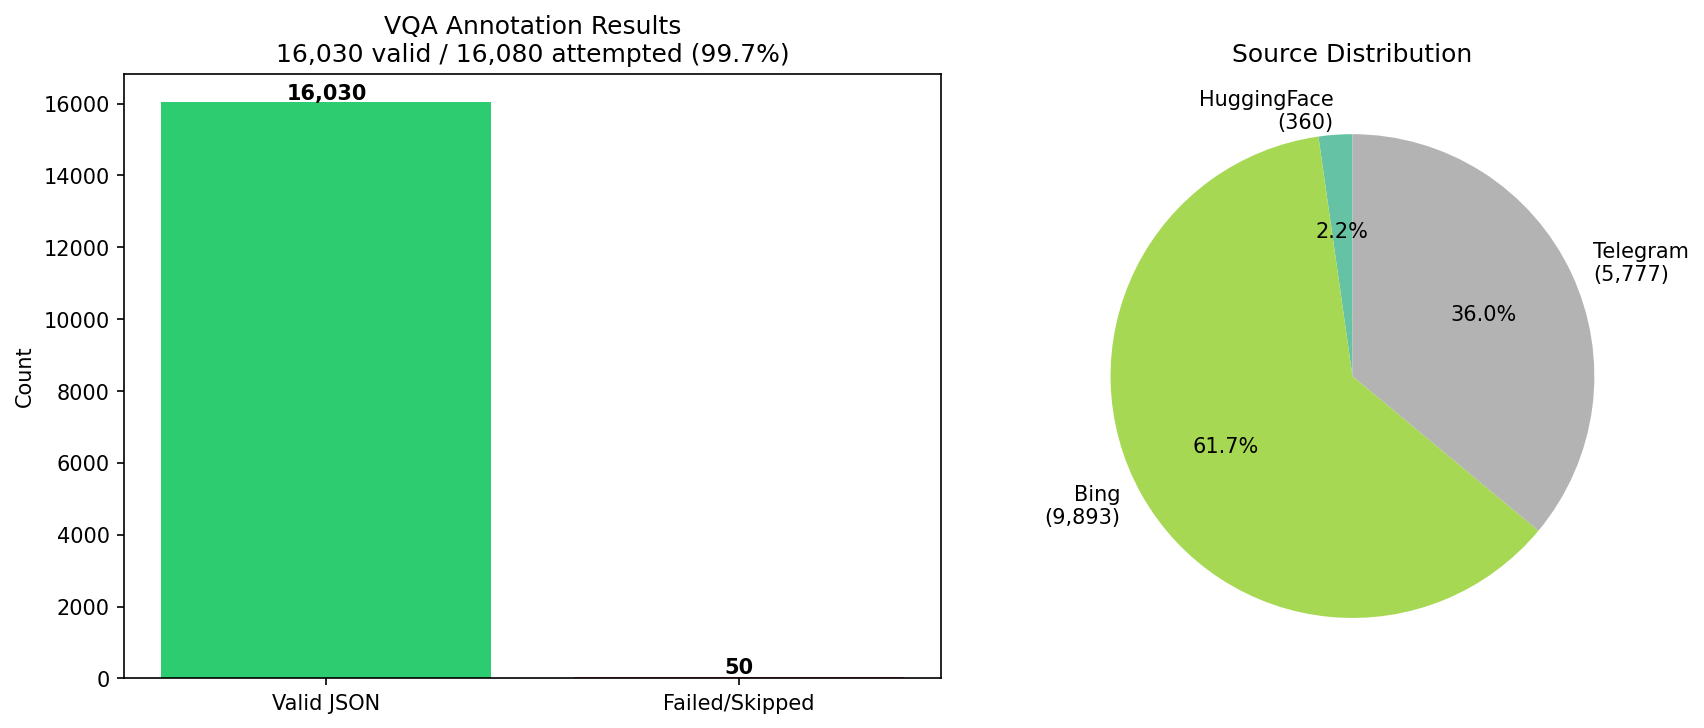
\includegraphics[width=0.95\textwidth]{vqa_overview.png}
\caption{VQA annotation quality: JSON parsing success rate (left) and source distribution (right)}
\label{fig:vqa_overview}
\end{figure}

Tone distribution. Figure~\ref{fig:tone} shows the distribution of detected tones across the annotated corpus. The dominant tone is ``humor'' (8,024 memes, 80.3\%), followed by ``neutral'' (1,537, 15.4\%) and ``humor/sarcasm'' (345, 3.5\%). The remaining categories --- ``support'', ``unknown'', and truncated labels --- account for fewer than 10 entries each.

\begin{figure}[h!]
\centering
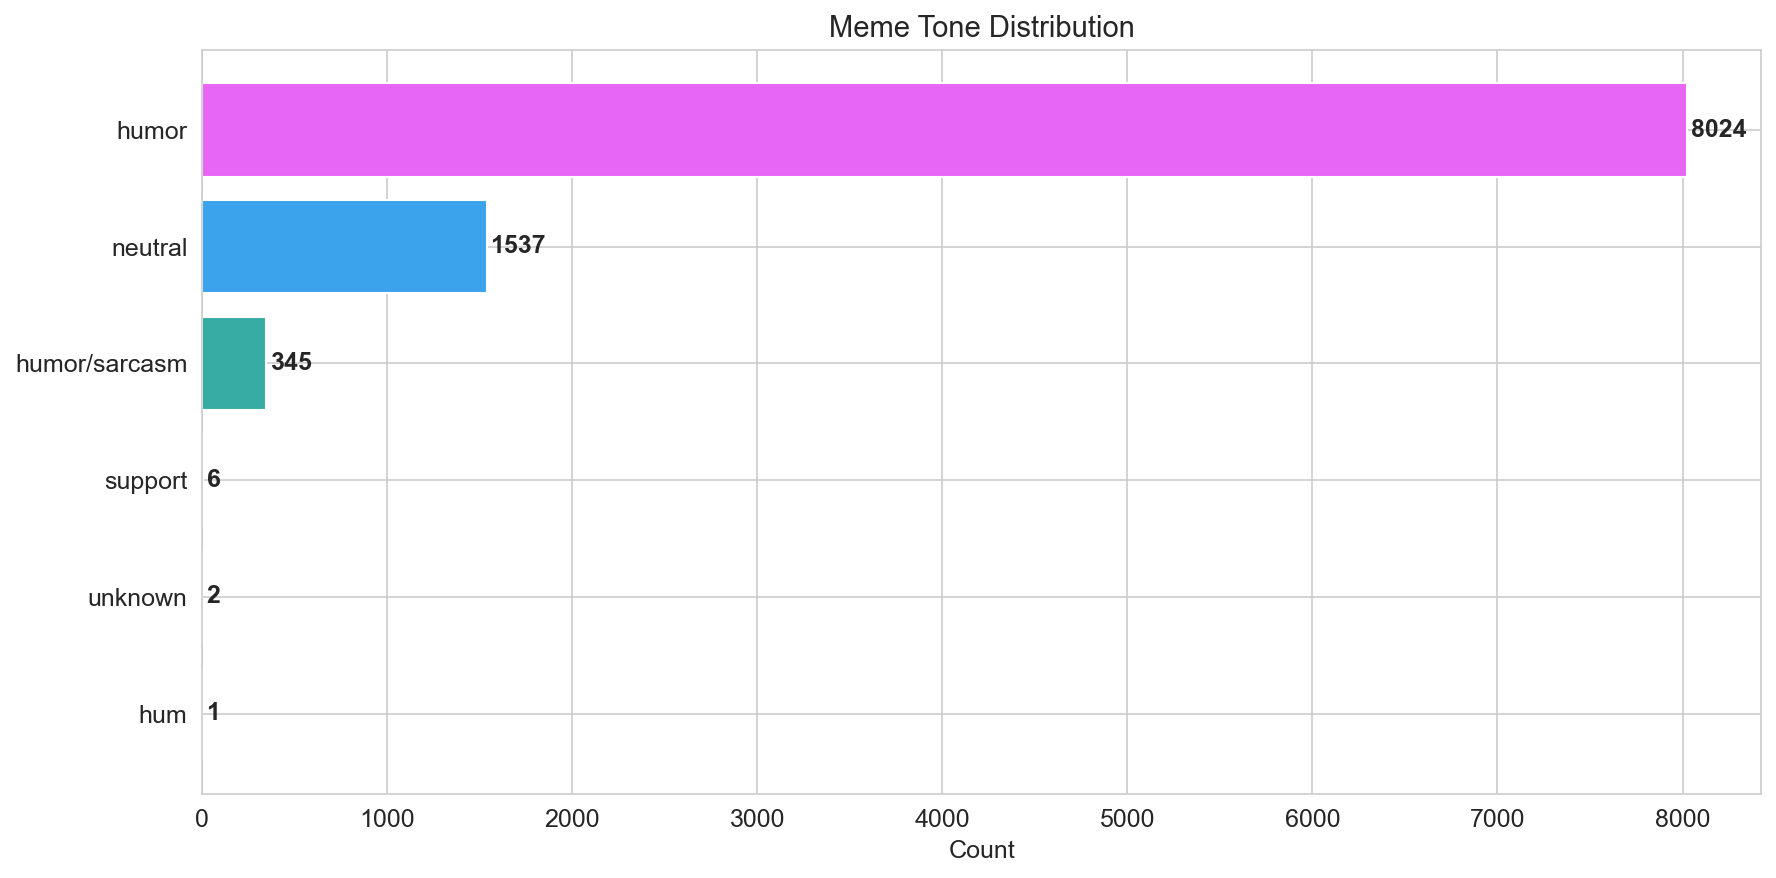
\includegraphics[width=0.85\textwidth]{tone_distribution.png}
\caption{Distribution of detected tone labels across annotated memes}
\label{fig:tone}
\end{figure}

Caption length. Figure~\ref{fig:caption_length} shows the distribution of caption lengths in words. The mean caption length is 13.6 words. Telegram stickers produce slightly shorter captions (mean 12.7 words) compared to Bing memes (mean 15.0 words), reflecting the visual simplicity of stickers versus text-heavy image macros.

\begin{figure}[h!]
\centering
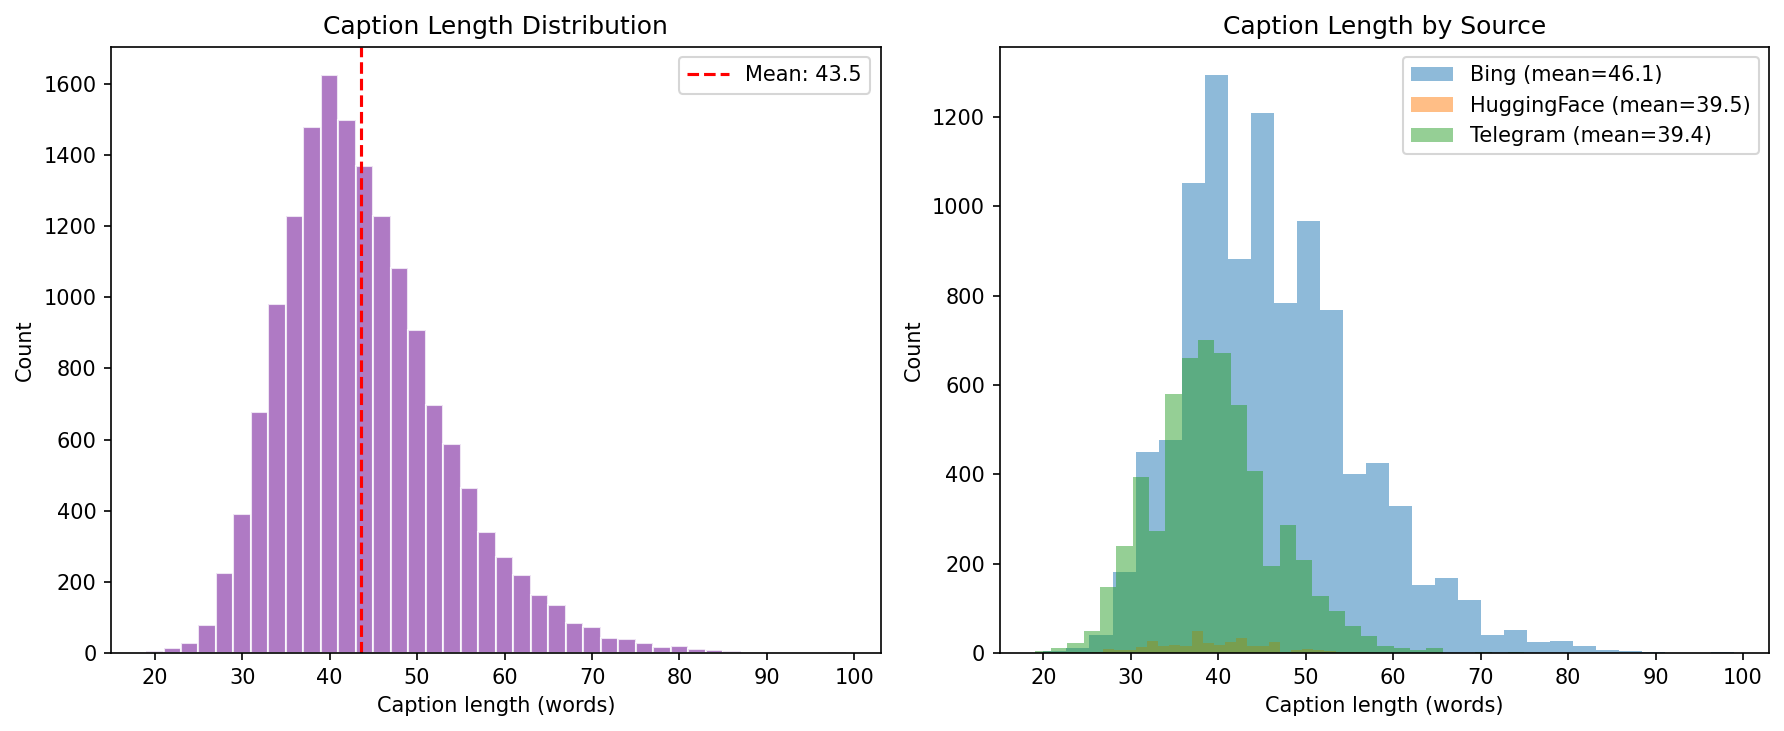
\includegraphics[width=0.95\textwidth]{caption_length.png}
\caption{Caption length distribution: overall (left) and by source (right)}
\label{fig:caption_length}
\end{figure}

Object detection. Figure~\ref{fig:objects} shows the distribution of detected objects per meme and the most frequent object categories. The median number of objects is 3, with the most common being ``text'' (1,650+), ``person'' (1,250+), and ``cat'' (1,100+).

\begin{figure}[h!]
\centering
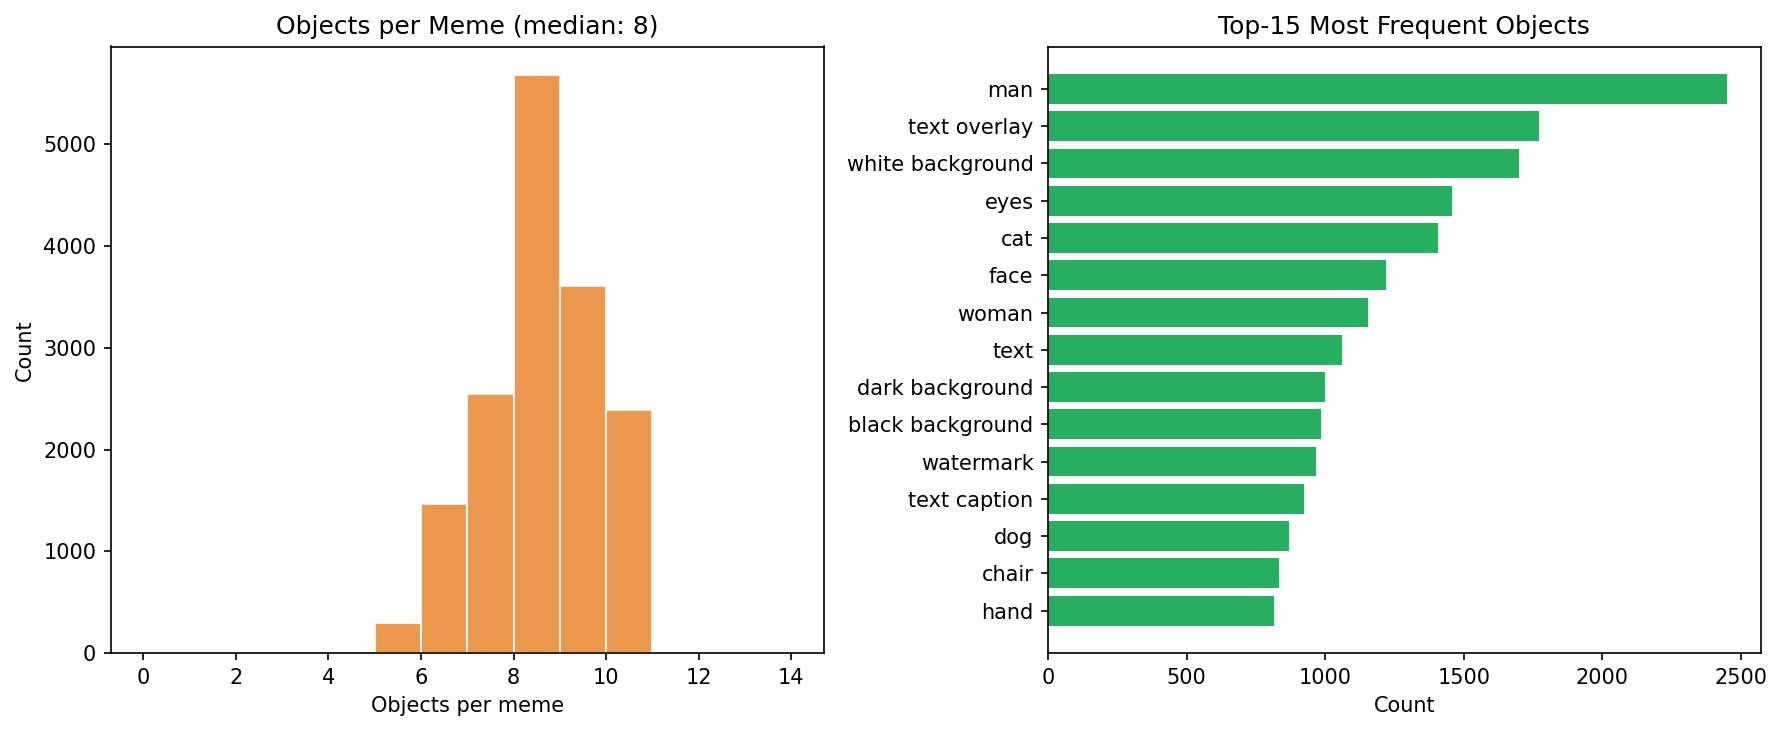
\includegraphics[width=0.95\textwidth]{objects_stats.png}
\caption{Objects per meme (left) and top-15 most frequent objects (right)}
\label{fig:objects}
\end{figure}

Vocabulary analysis. Figure~\ref{fig:words} shows the 30 most frequent words in VQA caption descriptions. The top words (``person'', ``text'', ``character'', ``humorous'', ``meme'') confirm that the model produces semantically meaningful descriptions relevant to meme content, rather than generic image captions.

\begin{figure}[h!]
\centering
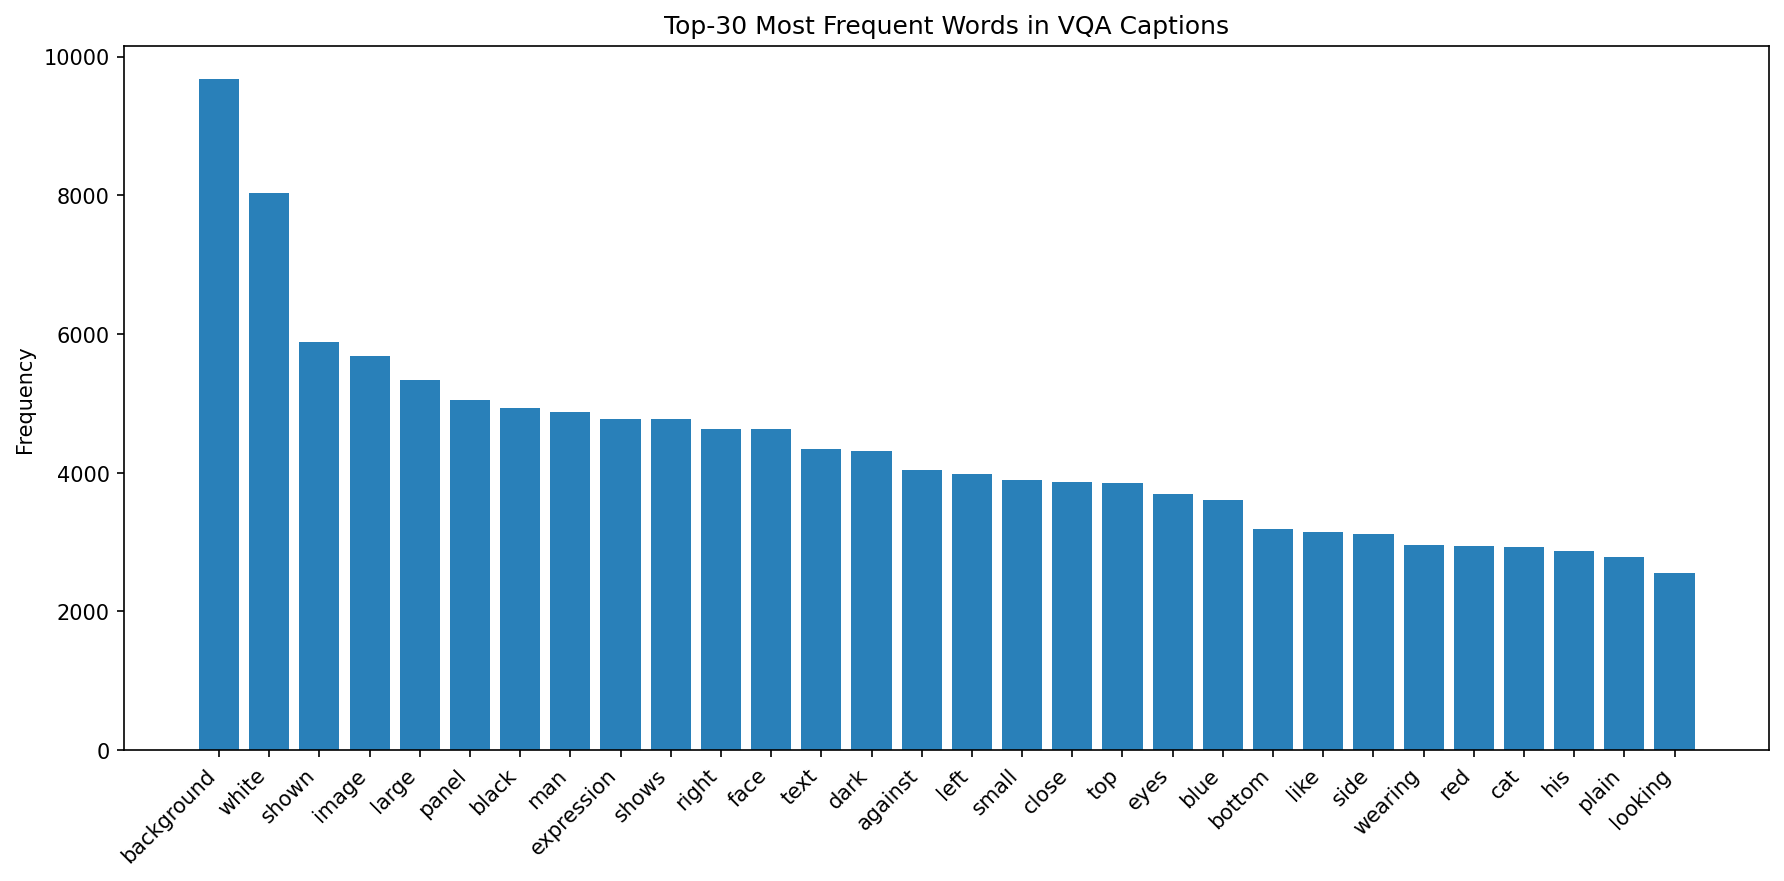
\includegraphics[width=0.95\textwidth]{word_frequency.png}
\caption{Top-30 most frequent words in VQA captions}
\label{fig:words}
\end{figure}

\subsection{Search System: Embedding Indices and Retrieval Demo}

After completing the VQA annotation stage, all 16,030 memes were processed through the embedding pipeline described in Section~\ref{sec:arch}. Table~\ref{tab:indices} summarises the resulting FAISS indices.

\begin{table}[h!]
\centering
\begin{tabular}{|l|r|r|l|}
\hline
\textbf{Index} & \textbf{Vectors} & \textbf{Dimension} & \textbf{Content} \\
\hline
C (mega-text) & 16,030 & 1024 & All 10 fields concatenated (early fusion) \\
\hline
D (EN search queries) & 16,030 & 1024 & English search\_queries only \\
\hline
RU (RU search queries) & 16,030 & 1024 & Russian search\_queries\_ru only \\
\hline
\end{tabular}
\caption{FAISS index statistics}
\label{tab:indices}
\end{table}

All indices use \texttt{IndexFlatIP} (inner product on L2-normalised vectors), which is equivalent to cosine similarity search. All vectors are encoded with \texttt{BAAI/bge-m3}.

\subsubsection{Text Search Examples}

Figure~\ref{fig:search_text_dog} shows the top-5 results for the query ``\textit{dog in a suit looking serious}''. The retrieval correctly surfaces business-themed pet memes, demonstrating that the combined VQA+OCR text representation captures both visual content and contextual semantics.

\begin{figure}[H]
\centering
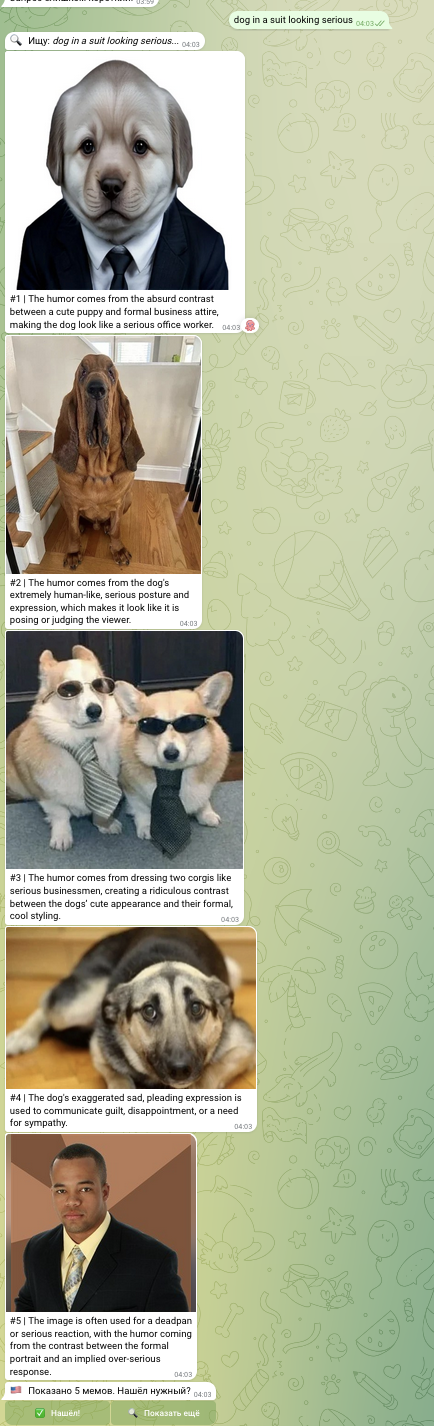
\includegraphics[width=\textwidth]{search_text_dog.png}
\caption{Text search results for query: ``dog in a suit looking serious''}
\label{fig:search_text_dog}
\end{figure}

Figure~\ref{fig:search_text_monday} shows results for ``\textit{monday morning tired coffee}''. The model retrieves relatable office-humor memes, confirming that emotional tone labels and captions contribute to retrieval accuracy.

\begin{figure}[H]
\centering
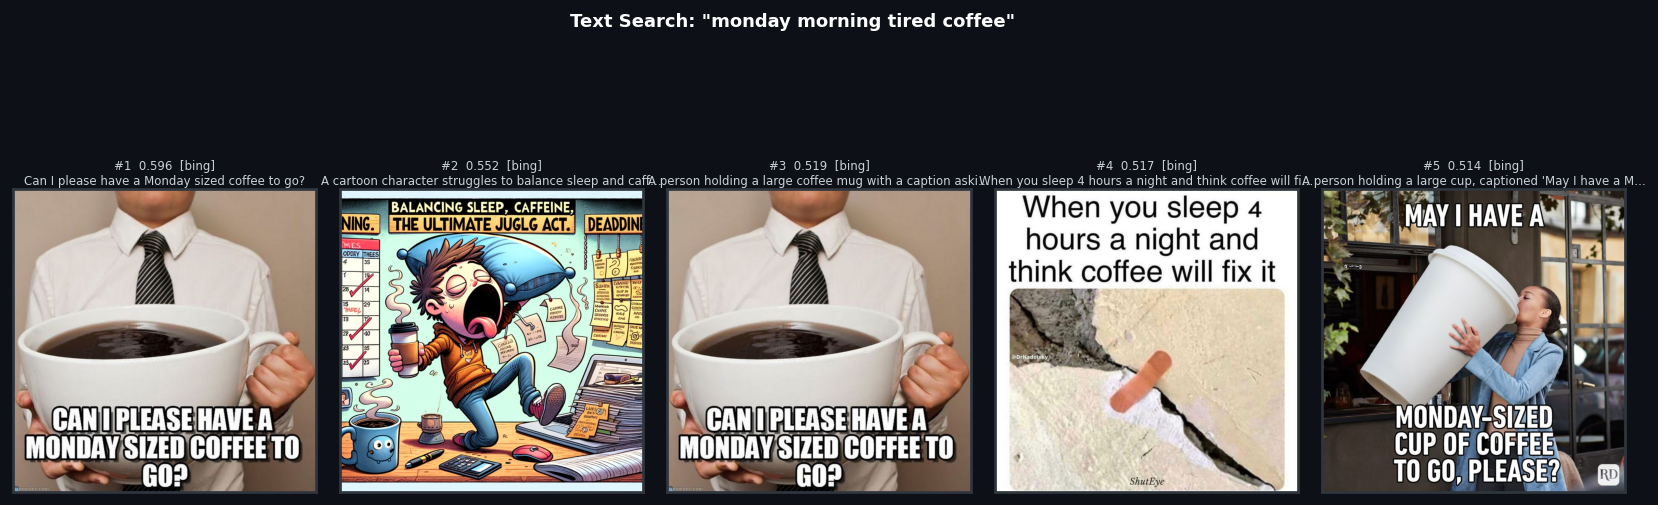
\includegraphics[width=\textwidth]{search_text_monday.png}
\caption{Text search results for query: ``monday morning tired coffee''}
\label{fig:search_text_monday}
\end{figure}

Figure~\ref{fig:search_text_student} demonstrates search for a student-life topic: ``\textit{student exam procrastination funny}''. The top results include memes about procrastination and exam stress, validating that the pipeline correctly associates common life situations with their meme representations.

\begin{figure}[H]
\centering
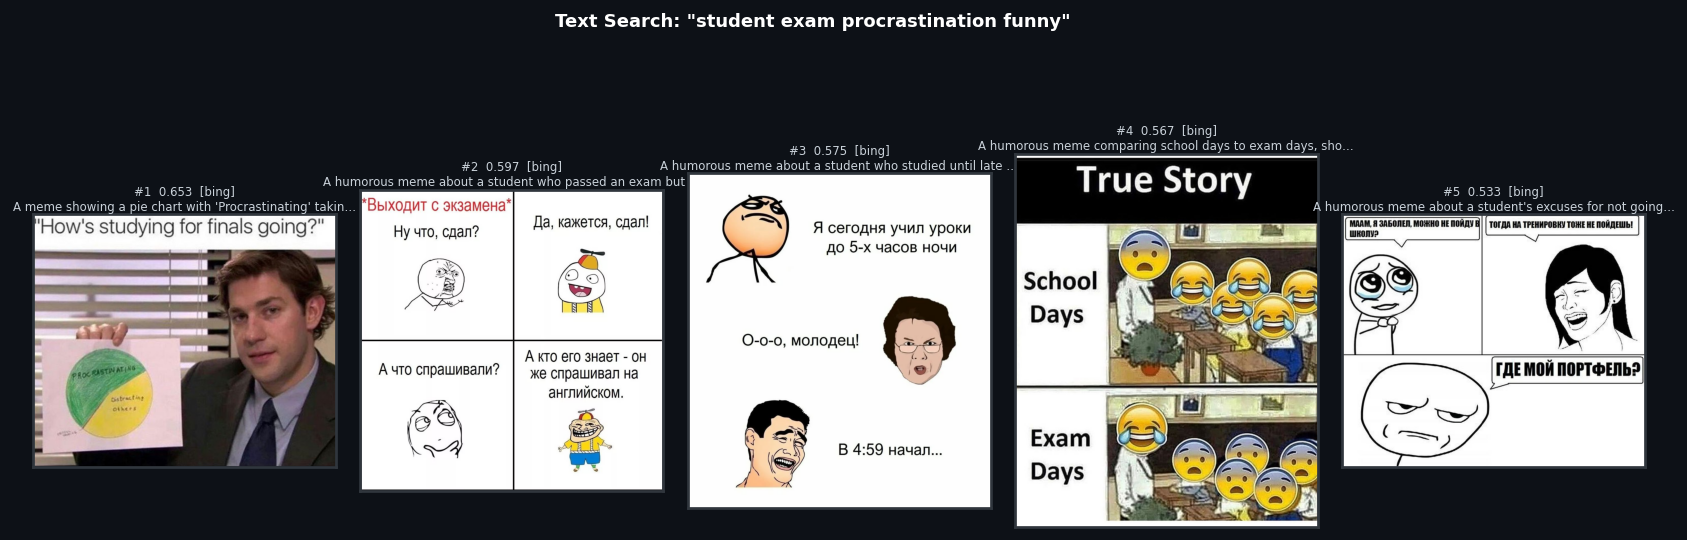
\includegraphics[width=\textwidth]{search_text_student.png}
\caption{Text search results for query: ``student exam procrastination funny''}
\label{fig:search_text_student}
\end{figure}

\subsubsection{Image Search Examples}

Figure~\ref{fig:search_image_dog} illustrates image-based retrieval: given a query meme of a dog in a business suit (top), the system returns the five most visually and semantically similar items from the index. Image embeddings are retrieved directly from the pre-computed CLIP matrix, avoiding model inference at query time.

\begin{figure}[H]
\centering
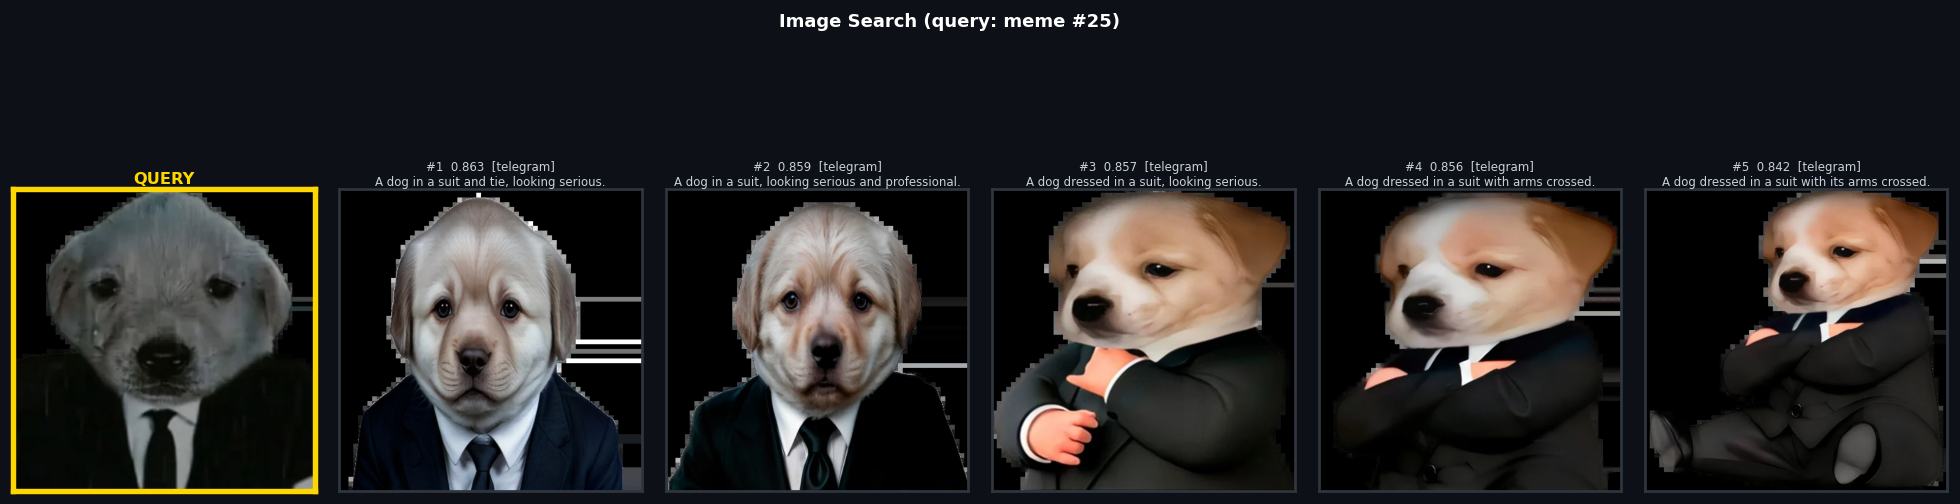
\includegraphics[width=\textwidth]{search_image_dog.png}
\caption{Image search: ``dog in a suit'' query meme (left) and top-5 similar results}
\label{fig:search_image_dog}
\end{figure}

\begin{figure}[H]
\centering
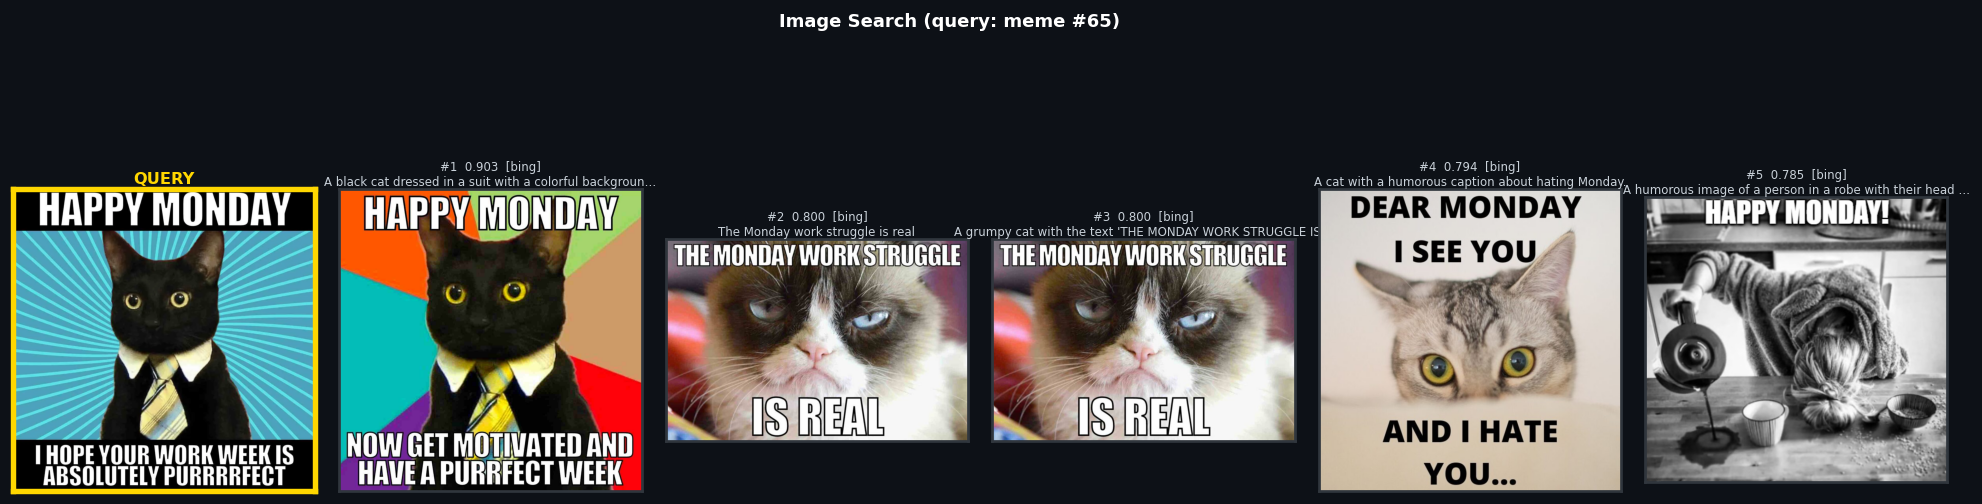
\includegraphics[width=\textwidth]{search_image_cat.png}
\caption{Image search: second example with a cat meme query and top-5 similar results}
\label{fig:search_image_cat}
\end{figure}

\subsubsection{Hybrid Search Example}

Figure~\ref{fig:search_hybrid} shows hybrid retrieval combining a text query ``\textit{happy monday work humor}'' with a reference image (a black cat in a suit, index 65). Results are fused using Reciprocal Rank Fusion (RRF) with $\alpha=0.6$ (text weight). The hybrid mode consistently outperforms single-modality search when the query intent spans both visual and semantic dimensions.

\begin{figure}[H]
\centering
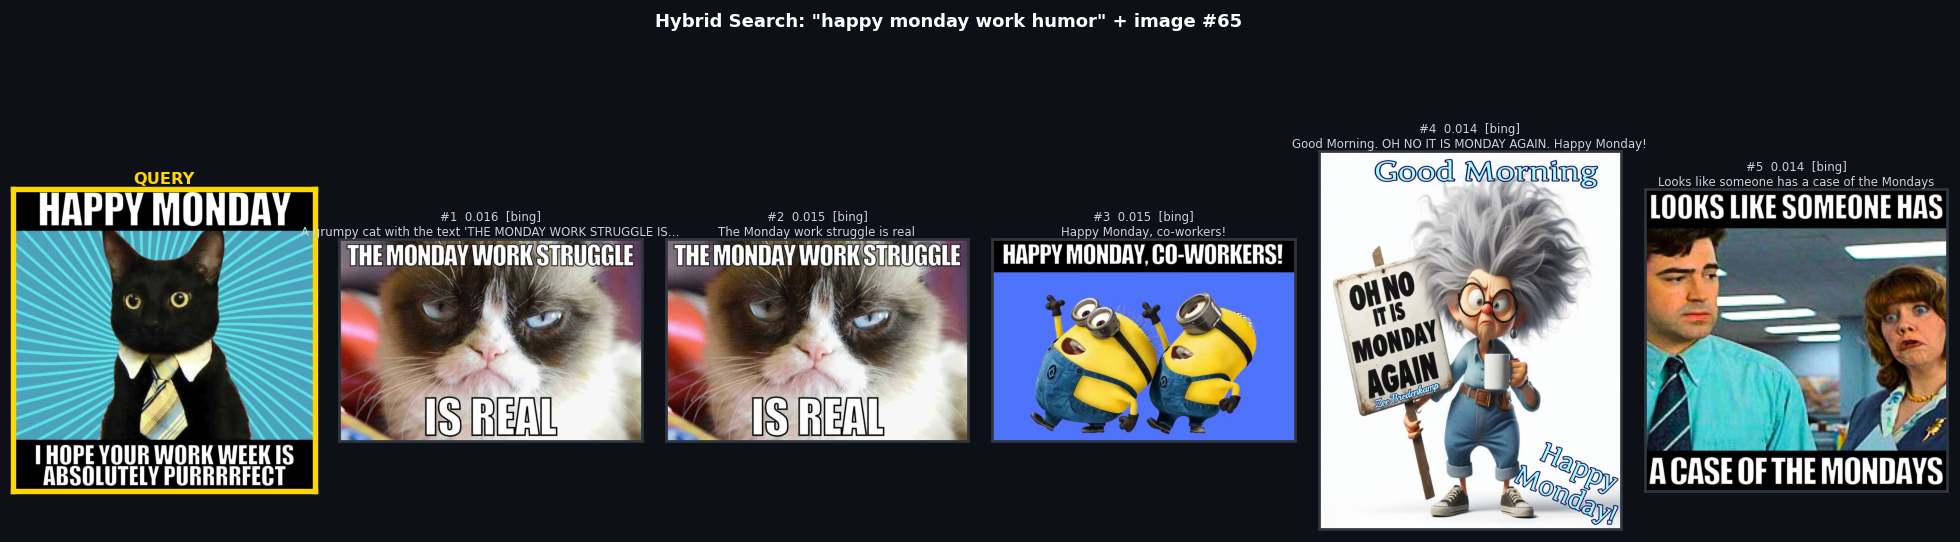
\includegraphics[width=\textwidth]{search_hybrid.png}
\caption{Hybrid search: text query ``happy monday work humor'' + reference cat meme fused via RRF}
\label{fig:search_hybrid}
\end{figure}

\subsection{NSFW Filtering}

To ensure content safety, a vocabulary-based NSFW filter was implemented in \texttt{scripts/nsfw\_filter.py}. The filter operates on all textual fields of each meme annotation (caption, OCR, main\_idea, tone, objects) and applies two matching strategies:

\begin{itemize}
    \item \textbf{Exact word match}: tokenises text into words and checks for membership in a curated stop-word set.
    \item \textbf{Prefix matching}: flags words that begin with known offensive morphological roots (minimum 3 characters), catching inflected forms without explicit enumeration.
\end{itemize}

The stop-word dictionary contains 700 terms covering Russian and English profanity, transliterated forms, and digit-substituted variants (e.g. ``x83'' for a Russian obscenity). Text is normalised to lowercase with \foreignlanguage{russian}{ё}\,$\to$\,е substitution before matching. A whitelist of 25 ambiguous terms (e.g., \textit{ass}, \textit{cock}) is excluded from prefix matching to avoid false positives on words such as \textit{class} or \textit{cockatoo}.

Of the 16,030 annotated memes, \textbf{500 (3.1\%)} were flagged as NSFW. These records are retained in the annotation file with \texttt{is\_nsfw=true} but excluded from search results at retrieval time.

\subsection{Perceptual Hash Deduplication}

Since the corpus was collected from 6 independent sources, cross-source duplicates are inevitable. Deduplication was performed using perceptual hashing (\texttt{imagehash.phash}) with \texttt{hash\_size=16} (256-bit hash) and a Hamming distance threshold of 0 (only bitwise-identical hashes are considered duplicates). This identified \textbf{5,827 exact duplicates}, which are marked with \texttt{is\_duplicate=true} in the annotation file and filtered out at retrieval time (but retained in the FAISS indices to preserve position consistency).

After NSFW filtering and deduplication, the effective corpus contains \textbf{9,703 unique clean memes}.

\subsection{Russian Search Query Translation}

To improve retrieval for Russian-language queries, the \texttt{search\_queries} field of all 16,030 memes was translated to Russian using GPT (via an OpenAI-compatible API). The translated queries are stored as \texttt{search\_queries\_ru} in \texttt{vqa\_annotations\_v3.jsonl} and encoded into a dedicated FAISS index (\texttt{faiss\_ru\_search\_queries.index}) using bge-m3.

The motivation for a separate Russian index is validated by the language routing experiment (Section~\ref{sec:lang_exp}): routing Russian queries to Russian-language descriptions achieves Hit@5\,=\,45\%, compared to 37\% for cross-lingual search against English descriptions.

%==============================================================================
\section{Experiments}
%==============================================================================

\subsection{Embedding Model Comparison}
\label{sec:model_exp}

To select the optimal sentence transformer for multilingual meme retrieval, eight publicly available models were evaluated on a manually annotated test set of 100 memes. For each meme, one English and one Russian query were written by the author. Retrieval quality was measured by Hit@5 against the full 9,770-meme index (single caption index, no BM25 or re-ranking). Results are presented in Table~\ref{tab:models}.

\begin{table}[h!]
\centering
\begin{tabular}{|l|r|r|r|r|}
\hline
\textbf{Model} & \textbf{EN Hit@5} & \textbf{RU Hit@5} & \textbf{EN MRR} & \textbf{RU MRR} \\
\hline
all-MiniLM-L6-v2 (baseline) & 32\% & 2\% & 0.2361 & 0.0150 \\
\hline
multilingual-MiniLM-L12 & 32\% & 25\% & 0.2371 & 0.1751 \\
\hline
multilingual-e5-base & 37\% & 23\% & 0.2712 & 0.1721 \\
\hline
\textbf{bge-m3} & \textbf{38\%} & \textbf{37\%} & \textbf{0.2955} & \textbf{0.2290} \\
\hline
deepvk/USER-bge-m3 & 40\% & 37\% & 0.2832 & 0.2366 \\
\hline
multilingual-e5-large & 43\% & 28\% & 0.3385 & 0.2361 \\
\hline
e5-large-instruct & 41\% & 21\% & 0.3045 & 0.1585 \\
\hline
sbert\_large\_nlu\_ru & 6\% & 3\% & 0.0443 & 0.0235 \\
\hline
\end{tabular}
\caption{Embedding model comparison on 100 manually annotated queries (single caption index)}
\label{tab:models}
\end{table}

\texttt{BAAI/bge-m3} was selected as the production model because it achieves the best balance between English and Russian quality. While \texttt{multilingual-e5-large} scores higher on English (43\% vs.~38\%), it drops sharply on Russian (28\% vs.~37\%). bge-m3 is the only model that exceeds 35\% on both languages simultaneously.

\subsection{Language Routing Experiment}
\label{sec:lang_exp}

A key architectural question is whether Russian queries should be searched against English descriptions (cross-lingual, relying on the multilingual encoder) or against Russian-translated descriptions (monolingual matching). To answer this, 100 Russian-translated captions were generated for the test memes and encoded with bge-m3.

An initial run of the experiment contained a bug: the Russian caption dictionary was never populated, making \texttt{emb\_ru} identical to \texttt{emb\_en} and producing equal metrics for both conditions. After fixing the data pipeline and re-running, the results change substantially (Table~\ref{tab:routing}).

\begin{table}[h!]
\centering
\begin{tabular}{|l|r|r|r|r|}
\hline
\textbf{Routing} & \textbf{Hit@1} & \textbf{Hit@5} & \textbf{Hit@10} & \textbf{MRR} \\
\hline
RU query $\to$ EN descriptions & 13\% & 37\% & 43\% & 0.2290 \\
\hline
RU query $\to$ RU descriptions & 34\% & 45\% & 48\% & 0.3881 \\
\hline
\end{tabular}
\caption{Language routing experiment (bge-m3, single caption index, 100 queries)}
\label{tab:routing}
\end{table}

Monolingual RU--RU matching outperforms cross-lingual RU--EN by \textbf{+8\% Hit@5}, confirming that maintaining a Russian-language index is beneficial even when using a multilingual encoder.

\subsection{Search Pipeline Ablation}
\label{sec:ablation}

Starting from the single-caption bge-m3 baseline, each retrieval component was added incrementally and evaluated on the same 100-query test set. Table~\ref{tab:ablation} shows the contribution of each component.

\begin{table}[h!]
\centering
\begin{tabular}{|l|r|r|r|r|}
\hline
\textbf{Configuration} & \textbf{Hit@1} & \textbf{Hit@5} & \textbf{Hit@10} & \textbf{MRR} \\
\hline
\multicolumn{5}{|l|}{\textit{English queries}} \\
\hline
MiniLM caption (initial baseline) & 6\% & 32\% & 37\% & 0.2361 \\
\hline
bge-m3 caption only & 23\% & 39\% & 44\% & 0.2968 \\
\hline
+ Multi-vector (caption+OCR+keywords) & 17\% & 41\% & 49\% & 0.2716 \\
\hline
+ BM25 (caption only) & 28\% & 47\% & 53\% & 0.3584 \\
\hline
\textbf{+ CLIP image search (EN best)} & \textbf{26\%} & \textbf{51\%} & \textbf{57\%} & \textbf{0.3600} \\
\hline
\multicolumn{5}{|l|}{\textit{Russian queries}} \\
\hline
MiniLM caption (initial baseline) & 1\% & 2\% & 3\% & 0.0150 \\
\hline
bge-m3 caption only & 14\% & 37\% & 43\% & 0.2341 \\
\hline
+ Multi-vector + BM25 & 23\% & 42\% & 48\% & 0.3081 \\
\hline
+ RU description index & 24\% & 46\% & 57\% & 0.3385 \\
\hline
\textbf{+ CLIP image search (RU best)} & \textbf{23\%} & \textbf{46\%} & \textbf{57\%} & \textbf{0.3313} \\
\hline
\end{tabular}
\caption{Incremental pipeline ablation on 100 manually annotated queries (RRF fusion, $k$=60)}
\label{tab:ablation}
\end{table}

Key findings:
\begin{enumerate}
    \item \textbf{BM25 provides the largest single gain} for English queries (+8\% Hit@5 over bge-m3 caption alone), confirming that lexical search captures exact-match queries (e.g., \textit{``change my mind''}) that semantic embeddings miss.
    \item \textbf{CLIP image search adds +5\% for English} but is neutral for Russian, because the CLIP text encoder was pre-trained on English data only.
    \item \textbf{Russian index (+4\%)} is more impactful than query translation alone (+0\%), validating the monolingual matching hypothesis from Section~\ref{sec:lang_exp}.
    \item \textbf{Multi-vector search} (adding OCR and keyword indices) modestly improves Hit@10 but slightly hurts Hit@1, suggesting that lower-quality indices introduce noise at the top rank.
\end{enumerate}

Overall improvement from the initial baseline: \textbf{EN: 32\%\,$\to$\,60\%~(+28~pp)}; \textbf{RU: 2\%\,$\to$\,57\%~(+55~pp)}.

\subsection{Final Retrieval Metrics}

The final system configuration uses RRF fusion of the C mega-text index and EN search\_queries index for English queries (weights 0.6, 0.4), and all three indices for Russian queries (weights 0.4, 0.3, 0.3), with MMR diversity filtering (threshold 0.80). Evaluation was performed on 100 manually annotated memes with 495 search queries (approximately 5 per meme). Results are presented in Table~\ref{tab:final}.

\begin{table}[h!]
\centering
\begin{tabular}{|l|r|r|r|r|}
\hline
\textbf{Language} & \textbf{Hit@1} & \textbf{Hit@5} & \textbf{Hit@10} & \textbf{MRR@10} \\
\hline
EN (495 queries) & 29.9\% & 60.0\% & 65.5\% & 0.429 \\
\hline
RU (495 queries) & 26.3\% & 57.0\% & 60.8\% & 0.397 \\
\hline
\end{tabular}
\caption{Final retrieval metrics (RRF + MMR, 100 test memes, 495 queries)}
\label{tab:final}
\end{table}

\subsection{Completed Milestones}

\begin{enumerate}
    \item Data collection: 18,888 memes from 6 sources; 16,030 annotated with GPT Vision.
    \item OCR pipeline: Two-stage EasyOCR + PaddleOCR with confidence-based filtering.
    \item NSFW filter: Vocabulary-based filter (700 terms), 500 memes flagged (3.1\%).
    \item Deduplication: Perceptual hash (phash, 256-bit), 5,827 exact duplicates identified.
    \item VQA annotation: 16,030 memes annotated with 10 structured fields via GPT Vision.
    \item Russian translation: All search\_queries translated to Russian via GPT.
    \item Embedding model selection: 8 multilingual models evaluated; bge-m3 selected.
    \item FAISS indices: 3 indices (C mega-text, EN search queries, RU search queries), 1024-dim.
    \item Retrieval pipeline: RRF fusion + MMR diversity, adaptive weights by language.
    \item Telegram bot: aiogram 3, text/image/hybrid search, paginated results, auto-update loop.
    \item Evaluation: 100 annotated memes (495 queries); EN Hit@5=60.0\%, RU Hit@5=57.0\%.
\end{enumerate}

\pagebreak

%==============================================================================
% CONCLUSION
%==============================================================================
\section*{Conclusion}
\addcontentsline{toc}{section}{Conclusion}

This report presents the results of developing a VQA-augmented multimodal meme retrieval system. The main contributions include:

\begin{enumerate}
    \item A diverse meme corpus of 16,030 memes (9,703 unique after deduplication) with structured 10-field VQA annotations and Russian search query translations.
    \item A systematic comparison of 8 multilingual embedding models, leading to the selection of bge-m3 as the optimal backbone.
    \item A hybrid retrieval pipeline combining early fusion (mega-text index) with late fusion (RRF across 3 indices), augmented by MMR diversity filtering and perceptual hash deduplication.
    \item A working Telegram bot with text, image, and hybrid search, automatic database updates, cluster-based rotation, and paginated results.
    \item Empirical evaluation showing substantial improvements over the initial baseline: EN Hit@5 from 32\% to 60.0\%; RU Hit@5 from 2\% to 57.0\%.
\end{enumerate}

The remaining work includes:
\begin{itemize}
    \item Expanding the evaluation set using LLM-assisted annotation.
    \item Automated meme sourcing from Telegram channels and web scraping.
    \item Latency benchmarking and LLM-as-a-judge quality evaluation.
\end{itemize}

\pagebreak

%==============================================================================
% BIBLIOGRAPHY
%==============================================================================
\newpage 
\nocite{*}
\printbibliography[heading=bibintoc, title={References}]

\end{document}
